\documentclass{amsart}
\usepackage{amsfonts, amsthm, amssymb, amsmath}
\usepackage{mathtools}
\usepackage{graphicx,caption,subcaption}
\usepackage{comment}
\usepackage{xcolor}
\usepackage{tikz}
%\usetikzlibrary{decorations.markings,arrows.meta,calc,fit,quotes,cd,math,external}
\usetikzlibrary{
  matrix,
  arrows,
  arrows.meta,
  calc,
  fit,
  quotes,
  cd,
  math,
  external,
  shapes,
  decorations.markings,
  decorations.pathreplacing,
  patterns,
  decorations.pathmorphing
}

\usepackage{url}
\usepackage[inline]{enumitem}
	\setlist{itemsep=0em, topsep=0em, parsep=0em}
	\setlist[enumerate]{label=(\alph*)}
\usepackage[all,2cell]{xy}\UseAllTwocells\SilentMatrices
\usepackage[breaklinks=true]{hyperref}%John's choices, can change; previous choice \definecolor{hyperrefcolor}{rgb}{0,0,0.7}
\definecolor{darkgreen}{rgb}{0,0.45,0}
\definecolor{myurlcolor}{rgb}{0.6,0,0}
\definecolor{mycitecolor}{rgb}{0,0,0.8}
\definecolor{myrefcolor}{rgb}{0,0,0.8}
\hypersetup{colorlinks, linkcolor=myrefcolor, citecolor=darkgreen, urlcolor=myurlcolor,
final,linktoc=page}
\usepackage[capitalize]{cleveref}
\crefname{equation}{}{}
\crefname{item}{}{}
\crefname{prop}{Proposition}{Propositions}

%
% environments and counters
%

\newtheorem{thm}{Theorem}[section]
\newtheorem{cnj}[thm]{Conjecture}
\newtheorem{lem}[thm]{Lemma}
\newtheorem{prop}[thm]{Proposition}
\newtheorem{cor}[thm]{Corollary}

\theoremstyle{remark}
	\newtheorem{remark}[thm]{Remark}
	\newtheorem{notation}[thm]{Notation}

\theoremstyle{definition}
	\newtheorem{ex}[thm]{Example} 
	\newtheorem{defn}[thm]{Definition}

% math text formatting
\newcommand{\cat}[1]{\mathsf{#1}}

% common category names

\newcommand{\Set}{\cat{Set}}
\newcommand{\Grph}{\cat{Grph}}
\newcommand{\Cat}{\cat{Cat}}
\newcommand{\twoCat}{\cat{2Cat}}
\newcommand{\Adj}{\cat{Adj}}
\newcommand{\one}{\mathbf{1}}
\newcommand{\two}{\mathbf{2}}
\newcommand{\Fib}{\cat{Fib}}
\newcommand{\OpFib}{\cat{OpFib}}
\newcommand{\Corefl}{\cat{Corefl}}
\newcommand{\Rali}{\cat{Rali}}

\newcommand{\C}{\cat{A}}
\newcommand{\D}{\cat{X}}
\newcommand{\A}{\cat{A}}
\newcommand{\X}{\cat{X}}
\newcommand{\U}{U}
\newcommand{\Q}{Q}
\renewcommand{\L}{L}
\newcommand{\R}{R}
\renewcommand{\P}{P}
\newcommand{\B}{\cat{B}}
\newcommand{\Y}{\cat{Y}}

\newcommand{\Cocart}{\mathrm{Cocart}}
\newcommand{\Cart}{\mathrm{Cart}}

\newcommand{\op}[1]{\operatorname{#1}}
\renewcommand{\t}[1]{\text{#1}}

\newcommand{\from}{\colon}
\newcommand{\xto}[1]{\xrightarrow{#1}}
\newcommand{\To}{\Rightarrow}
\newcommand{\Tto}{\Rrightarrow}
\newcommand{\bydef}{\coloneqq}
\newcommand{\define}{\textbf}%consider change to bold? or something else?

%
% math operators
%

\DeclareMathOperator{\Hom}{Hom}
\DeclareMathOperator{\id}{id}
\DeclareMathOperator{\ob}{Ob}
\DeclareMathOperator{\arr}{arr}
\DeclareMathOperator{\im}{im}
\DeclareMathOperator{\Aut}{Aut}
\DeclareMathOperator{\Bij}{Bij}
\DeclareMathOperator{\Sub}{Sub}
\DeclareMathOperator{\colim}{colim}
\newcommand{\iso}{\cong}

%
% tikz styles
%

% arrows for commuting diagram
\tikzset{
  cd/.style={
    ->,
    scale=6,
    >=angle 90,
    font=\scriptsize}
  }

% its us!

\definecolor{purple(x11)}{rgb}{0.5, 0.0, 0.5}
\newcommand{\chris}{\color{purple(x11)}}
\newcommand{\daniel}{\color{red}}

\begin{document}
\title{A note on Fibrations and Adjunctions}

\author{Daniel Cicala and Christina Vasilakopoulou} 
\address{update departments}
\email{update emails}

\begin{abstract}
Fibrations and Adjunctions rock.
\end{abstract}

\maketitle
% \tableofcontents


% TODO write intro

% ===============================================================
% Introduction


% ===============================================================
% Preliminaries. Basic def's and set notation. Include lemmas

\section{Preliminaries}\label{sec:preliminaries}

In this section, we present the necessary background for this paper
and take this opportunity to set our notation and conventions. One
convention we employ is the singular focus on opfibrations instead of
their dual, fibrations.  We cover two flavors of opfibrations,
Grothendieck and Street, and also present a lemma that relates
colimits in the fibres to colimits in the total category.

\subsection*{Grothendieck Opfibrations} % ~~~~~~~~~~~~~~~~~~~~

We recall some basic material from the theory of (Grothendieck) opfibrations; standard references include \cite{Handbook2,Grayfibredandcofibred,hermidaphd}. 

Fix a functor $\U \colon\X \to \A$. An object $x$ in $\X$ is said to
\define{be over} an object $a$ in $\A$ if $Ux=a$. The same terminology
applies for arrows. An arrow $\beta$ in $\X $ over an arrow
$f \from a \to b$ in $\A$ is called \define{cocartesian} if and only
if, for all $g \colon b \to b'$ in $\A$ and $\gamma \colon x\to y'$ in
$\X $ with $\U(\gamma) = g\circ f$, there exists a unique
$\delta \colon y\to y'$ in $\X$ such that $\U(\delta) = g$ and
$\gamma = \delta \circ \beta$ (see Figure \ref{fig:opfibration})
\begin{figure} 
  \fbox{
    \begin{minipage}{1.0\linewidth}
      \centering
  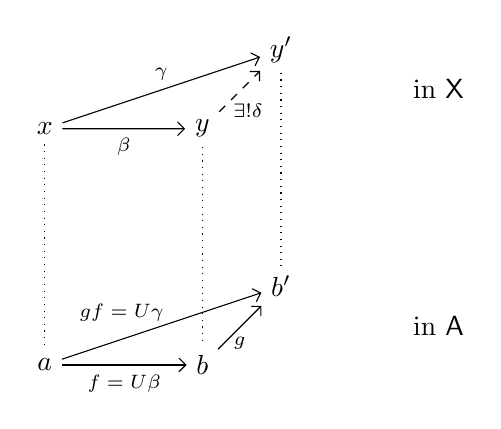
\begin{tikzpicture}
    \node (a) at (0,0) {$ a $};
    \node (b) at (2,0) {$ b $};
    \node (b') at (3,1) {$ b' $};
    \node (x) at (0,3) {$ x $};
    \node (y) at (2,3) {$ y $};
    \node (y') at (3,4) {$ y' $};
    \draw [cd] 
    (a) edge[] node[below]{$f=U\beta$} (b)
    (b) edge[] node[below]{$g$} (b')
    (a) edge[] node[above=3pt,pos=0.3]{$gf=U\gamma$} (b')
    (x) edge[] node[below]{$\beta$} (y)
    (y) edge[dashed] node[below=4pt,pos=0.7]{$\exists! \delta$} (y')
    (x) edge[] node[above]{$\gamma$} (y');
    \node () at (5,3.5) {in $ \X $};
    \node () at (5,0.5) {in $ \A $};
    \draw [dotted]
    (x) edge[] (a)
    (y) edge[] (b)
    (y') edge[] (b');
  \end{tikzpicture}
  \caption{Cocartesian Lifting}
  \label{fig:opfibration}
\end{minipage}
}
\end{figure}

For any object $a$ in $\A$, let $\X_a$ denote the \define{fibre} of $U$ over $a$, that is the subcategory of $\X$ that consists of the objects $x$ over $a$ and \define{vertical arrows} (those sent by $U$ to $1_a$). The functor $\U \colon \X \to \A$ is an \define{opfibration} if and only if, for all $f \colon a \to b$ in $\A$ and $x$ in $\X_a$, there is a cocartesian arrow $\beta$ with domain $x$ above $f$; it is called a \define{cocartesian lifting} of $b$ along $f$. The category $\A$ is called the \define{base} of the opfibration, and $\X $ its \define{total category}.
Of course, this is a dual notion to that of a \define{fibration}.

For any opfibration $\U\colon \X \to\A$, we may use the axiom of choice to select a cocartesian lift $\Cocart(f,x)\colon x\to f_!(x)$ of each $f\colon a\to b$ in $\A$ and $x$ in $X_a$. An opfibration equipped with a choice of cocartesian liftings is called a \define{cloven opfibration}.  Moving forward, we take all opfibration to be cloven. As a special case of the universal property, every arrow in the total category of an opfibration factorizes uniquely into a cocartesian arrow followed by a vertical arrow:
\begin{equation}\label{factor}
\begin{tikzpicture}[baseline=(current bounding box.center)]
  \node (a) at (0,0) {$ a $};
  \node (b) at (3,0) {$ b $};
  \node (x) at (0,3) {$ x $};
  \node (y) at (3,3) {$ y $};
  \node (fx) at (3,2) {$ f_!x $};
  \draw [cd]
    (a) edge[] node[below]{$f$} (b)
    (x) edge[] node[above]{$\gamma$} (y)
    (x) edge[] node[below=5pt]{$\Cocart(f,x)$} (fx)
    (fx) edge[dashed] node[right]{$\delta$} (y);
  \node () at (5,2.5) {in $ \X $};
  \node () at (5,0) {in $ \A $};
  \draw [dotted]
    (x) edge[] (a)
    (fx) edge[] (b);  
\end{tikzpicture}
\end{equation}

The choice of cocartesian liftings in a cloven opfibration induces a \define{reindexing functor} between the fibre categories
\begin{equation}\label{reindexing}
 f_!\colon\X_a\to\X_b,
\end{equation}
one for each $f\colon a\to b$ in the base category. It can be verified by the cocartesian lifting property that $(1_a)_!\cong1_{\X_a}$ and $(f\circ g)_!\cong f_!\circ g_!$. 

To relate opfibrations to right adjoints, we use the following lemma which clarifies the relationship between the existence of colimits in the total category of an opfibration to the existence of those colimits in the fibres. For more details and a proof of the following result, see \cite[Cor. 3.7]{FibredAdjunctions}.

\begin{lem}\label{lem:fibrewiselimits}
  Suppose $\cat{J}$ is a small category and $\U\colon\X\to\A$ is an
  opfibration whose base $\A$ has $\cat{J}$-colimits. The following
  are equivalent:
\begin{enumerate}
 \item all fibres have $\cat{J}$-colimits, and the reindexing functors preserve them; \label{it:2}
 \item the total category $\X$ has $\cat{J}$-colimits, and $\U$ (strictly) preserves them.
\end{enumerate}
\end{lem}

\begin{remark}
  This lemma still holds when $\U$ merely preserves colimits if the axiom of
  choice is assumed. To assuage those who are cautious about the axiom
  of choice, we discuss in Appendix \ref{lem:isofactid} several
  classes of functions that may safely be assumed to strictly preserve
  colimits.
\end{remark}

When condition \ref{it:2} holds, we typically say the opfibration has
\emph{opfibred $\cat{J}$-colimits} though, in principle, this does not
require a $\cat{J}$-cocomplete base.

\subsection{Street Opfibrations}

Typically, we ask for constructions in category theory to transport
across equivalent categories. Grothendieck opfibrations, in general,
do not have this property. That is, given a Grothendieck opfibration
$U \from \X \to \A$ and equivalence of categories $E \from \X' \to \X$
or $E' \from \A \to \A'$, neither $UE$ nor $E'U$ are necessarily
Grothendieck opfibrations.  Indeed, given an arrow $f \from a \to b$
in $\A$ with cocartesian lifting $\beta \from x \to y$, a Grothendieck
opfibration requires an equality $Uy=b$ which may weaken to an
isomorphism after extending $\U$ by an equivalence. Street
opfibrations avoid this defect. While they were originally defined
internally to 2-categories \cite{FibYon}, we restrict our attention $\Cat$.

\begin{defn}
  A functor $ U \from \X \to \A $ is a \define{Street opfibration} if,
  for any arrow $ f \from a \to b $ in $ \A $ and $ x $ over $ a $,
  there exists a cocartesian arrow $ \theta \from x \to y $ and an
  isomorphism $ h \from b \iso Uy $ such that $ fh = U\theta $ (see
  Figure \ref{fig:street_opfib})
\end{defn}

\begin{figure}[h]
  \fbox{
    \begin{minipage}{1.0\linewidth}
      \centering
    \begin{tikzpicture}[baseline=(current bounding box.center)]
    \node (a) at (0,0) {$ a $};
    \node (b) at (2,0) {$ b $};
    \node (Uy) at (3,1) {$ Uy $};
    \node (x) at (0,3) {$ x $};
    \node (y) at (3,3) {$ y $};
    \draw [cd] 
    (a) edge[] node[below]{$f$} (b)
    (b) edge[] node[below]{$h$} (Uy)
    (a) edge[] node[above=3pt,pos=0.3]{$U\beta$} (Uy)
    (x) edge[] node[above]{$\beta$} (y);
    \node () at (5,3) {in $ \X $};
    \node () at (5,0.5) {in $ \A $};
    \draw [dotted]
    (x) edge[] (a)
    (y) edge[] (Uy);
  \end{tikzpicture}
  \caption{Street Opfibration}
  \label{fig:street_opfib}
\end{minipage}
}
\end{figure}

The definition of ``cocartesian arrow'' here is the same used for
Grothendieck opfibrations. The isomorphism $ h $, which replaces an
equality in a Grothendieck opfibration, ensures that Street
opfibrations do transport across equivalences. 

In Section \ref{sec:groth-fibs-ralis}, we expose a relationship
between Street opfibrations and right adjoints for which we use a
generalized version of Lemma \ref{lem:fibrewiselimits}. In order to
prove this lemma, we first present several standard results and recall
the definition of an isofibration.

\begin{defn}
  A functor $U \from \X \to \A$ is an \define{isofibration} if, for
  every isomorphism $f \from Ux \to a$ in $\A$, there is an
  isomorphism $\hat{f} \from x \to x'$ in $\X$ such that $U\hat{f}=f$.
\end{defn}

\begin{lem} \label{lem:street_and_iso_is_groth} If a functor is a
  Street opfibration and an isofibration, then it is also a
  Grothendieck fibration.
\end{lem}

\begin{proof}
  Let $U \from\X \to \A$ be both a Street opfibration and
  isofibration. To an arrow $f \from Ux \to a$, we associate an
  cocartesian lifting $\theta \from x \to y$ and isomorphism
  $h \from a \to Uy$. Let $\hat{h^{-1}}$ be the invertible arrow in
  $\X$ over $h^{-1}$. The cocartesian arrow lift of $f$ is
  $\theta \hat{h^{-1}}$.
\end{proof}

\begin{lem} \label{lem:street_decomposed} A Street opfibration can be
  decomposed into a Grothendieck opfibration followed by an
  equivalence of categories.
\end{lem}

\begin{proof}
  There is a model structure on $\Cat$ whose weak equivalences are
  equivalences of categories and whose fibrations are isofibrations
  \cite{rezk}. Hence, we can decompose a Street opfibration into an
  isofibration followed by a equivalence of categories. The
  isofibration is equivalent to a Street opfibration so is itself a
  Street opfibration and therefore, by Lemma
  \ref{lem:street_and_iso_is_groth}, a Grothendieck opfibration.
\end{proof}

\begin{lem} \label{lem:street-fibrewise-limits}
  Suppose $ \cat{J} $ is a small category and $ U \from \X
  \to \A $ is a Street opfibration. If $ \A $ has $ \cat{J}
  $-colimits, the following are equivalent:
  \begin{enumerate}
  \item
    all fibres have $ \cat{J} $-colimits and the
    reindexing functors preserve them;
  \item
    $ \X $ has $ \cat{J} $-colimits and $ U $ preserves
    them.
  \end{enumerate}
\end{lem}

\begin{proof}
  Per Lemma \ref{lem:street_decomposed}, decompose $U$ into $H U'$
  where $U'$ is a Street opfibration and $H$ is an equivalence. The
  result follows by applying Lemma \ref{lem:fibrewiselimits} to $U'$.
\end{proof}

\subsection{Coreflectors and ralis}

The main results of this paper are a correspondence between the
Grothendieck and Street opfibrations and certain right adjoint
functors. In this section, we recall the definitions of these certain
right adjoints, ralis and coreflectors. These sorts of right adjoints
are closely related, with ralis having the stronger definition.

A \define{rali}, or right-adjoint-left-inverse, is the right adjoint
$\U$ portion of an adjunction $\L\dashv\U\colon\X\to\A$ that satisfies
the equation $UL=1_{\A}$ or, equivalently, has a unit consisting of
only identity arrows. If $\epsilon$ is the counit of a rali, then
$\U\epsilon$ and $\epsilon_\L$ are also identities. Also, the equation
$ULU=U$ holds. The term \define{lari}, or left-adjoint-right-inverse,
was introduced by Gray \cite{Grayfibredandcofibred}.

Just as a Street opfibration is a weaker version of a Grothendieck
opfibration, a coreflector is a weaker version of a rali.  This next
proposition gives defining properties for a coreflector.

\begin{prop}[{\cite[Prop.~3.4.1]{Handbook1}}]\label{prop:coreflection}
  The following are equivalent for an adjunction
  $\L\dashv\U\colon\X\to\A$:
  \begin{enumerate}
  \item the left adjoint $\L$ is full and faithful;
  \item the unit $\eta\colon1_\A\Rightarrow \U\L$ is an isomorphism.
 \end{enumerate}
 Under these conditions, $\U\epsilon$ and $\epsilon_\L$ are also
 isomorphisms.
\end{prop}

An adjuntion $\L\dashv\U$ satisfiying these properties is called a
\define{coreflection}, the right adjoint $\U$ a \define{coreflector}, and
$\A$ a \define{coreflective} subcategory of $\X$.


% ===============================================================
% Groth fibs and ralis. Examine relationship between.

\section{Grothendieck fibrations and ralis}
\label{sec:groth-fibs-ralis}

In this section, we investigate the relationship between Grothendieck opfibrations and right adjoints. We start by finding conditions under which an opfibration is a right adjoint.  We then find conditions under which a right adjoint is an opfibration. We conclude this section by exhibiting the correspondence by intersecting the respective conditions.

The following result is an answer to the question: when is an opfibration a right adjoint? It is dual to a proposition of Gray \cite[Prop. 4.4]{Grayfibredandcofibred}.

\begin{prop} \label{prop:opfibtolari} Let $\U \from \D \to \C$ be an  opfibration. Then $\U$ is a rali if its fibres have initial objects which are preserved by the reindexing functors.
\end{prop}

\begin{proof}
Denote by $\bot_a$ the initial object in fiber $\X_a$. Define a functor $\L \from \A \to \X$ as shown in the diagram
\begin{equation*}
  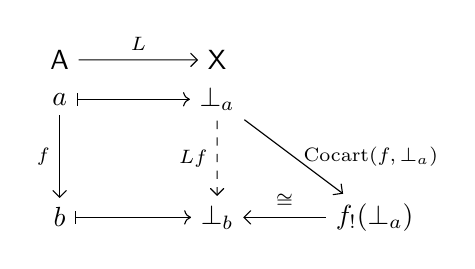
\begin{tikzpicture}
    \node (b) at (0,0) {$ b $};
    \node (botb) at (2,0) {$ \bot_b $};
    \node (f) at (4,0) {$ f_!(\bot_a) $};
    \node (a) at (0,1.5) {$ a $};
    \node (bota) at (2,1.5) {$ \bot_a $};
    \node (A) at (0,2) {$ \A $};
    \node (X) at (2,2) {$ \X $};
    \draw [cd] 
    (a) edge[] node[left]{$f$} (b)
    (bota) edge[dashed] node[left]{$Lf$} (botb)
    (bota) edge[] node[right]{$\Cocart(f,\bot_a)$} (f)
    (A) edge[] node[above]{$L$} (X)
    (f) edge[] node[above]{$\iso$} (botb) ;
    \draw [|->]
    (a) edge[] (bota)
    (b) edge[] (botb);
  \end{tikzpicture}
\end{equation*}

 % the below beautiful diagram was sacrificed for the sake of
% uniformity accross all diagrams and I don't know xypic
%
%
  
% \begin{tikzcd}[row sep=.05in,cells={anchor=east}]
%   \L\colon\A\ar[rr] && \X\;\; &\\
%   a\ar[rr,mapsto]\ar[dd,"f"'] && \bot_a\ar[dd,dashed,"\L f"']\ar[ddr,"{\Cocart(f,\bot_a)}"] & \\
% \hole \\
% b\ar[rr,mapsto] && \bot_b & f_!(\bot_a)\ar[l,"\iso"']
% \end{tikzcd}

where $f_!(\bot_a) \xto \bot_b$ arises from $f_!$ preserving initial objects. This assignment is functorial due to the universal properties of cocartesian liftings.

To show that $L$ is left adjoint to $\U$, it suffices to establish a natural bijection $\X(\L a,x)\cong\A(a,\U x)$ for any $a\in\A$, $x\in\X$. Indeed, each arrow in the total category $k\colon \L a\to x$ above $f=\U k$, factorizes uniquely (cf.~Diagram \ref{factor}) as
\begin{equation*}
  \begin{tikzpicture}[baseline=(current bounding box.center)]
    \node (a) at (0,0) {$ a $};
    \node (Ux) at (3,0) {$ Ux $};
    \node (bot) at (0,3) {$ \bot_a $};
    \node (x) at (3,3) {$ x $};
    \node (fbot) at (3,2) {$ f_!(\bot_a) $};
    \draw [cd]
      (a) edge[] node[below]{$f$} (Ux)
      (bot) edge[] node[above]{$k$} (x)
      (bot) edge[] node[below=6pt,pos=0.4]{$\Cocart(f,\bot_a)$} (fbot)
      (fbot) edge[dashed] node[right]{$s$} (x);
    \node () at (5,2.5) {in $ \X $};
    \node () at (5,0) {in $ \A $};
    \draw [dotted]
    (bot) edge[] (a)
    (fbot) edge[] (Ux);
  \end{tikzpicture}
\end{equation*}

% the below beautiful diagram was sacrificed for the sake of
% uniformity accross all diagrams and I don't know xypic
%
%
% \begin{displaymath}
% \xymatrix @C=.5in @R=.3in
% {\bot_a \ar @{.>}[dd]\ar[rr]^k \ar[drr]_-{\Cocart(f,\bot_a)} && x &\\
% && f_!(\bot_a) \ar @{-->}[u]_-s \ar @{.>}[d] & \textrm{in }\X \\
% a\ar[rr]_-{f} && \U x & \textrm{in }\A}
% \end{displaymath}
but since $f_!(\bot_a)\cong\bot_{\U x}$ is the initial object in the fibre above $\U x$, the arrow $s$ is in fact unique. As a result, every $k$ uniquely corresponds to some $f$ in that way, and this isomorphism is natural.

Finally, $\U$ is a left inverse of $\L$ because the unit of the adjunction $\eta\colon 1_\A \to \U\L$ is the identity natural transformation. Indeed, $\U\L a=U\bot_a=a$ and moreover, applying the natural bijection coming from the adjunction to \[\X (\bot_a,\bot_a)=\X (\L a,\L a)\cong\A(a,\U\L a)=\A (a,a)\] ensures that the identity on $\bot_a$ corresponds to the identity on $a$.
\end{proof}

Notice that because $\U$ is a right adjoint, it is slightly surprising that the existence of $\U$ is related to $U$ preserving initial objects. While this proposition uses reindexing functors to relate opfibrations and ralis, we can use Lemma \ref{lem:fibrewiselimits} to use a property of $U$ instead.

\begin{cor}
  An opfibration is a rali if the base category has and the functor strictly preserves the initial object.
\end{cor}

Next, we examine when a rali is an opfibration. The relevant condition is that a rali $U$ strictly preserves pushouts, choosen so that the pushouts strictly preserve identities. Strict preservation is a strong condition, but this can be safely assumed for a non-trivial class of functors.  We discuss this further in Appendix \ref{sec:choice_of_colimits}.

\begin{prop}\label{prop:laritoopfib}
  Suppose that $\U\colon\X\to\A$ is a rali. Then $\U$ is an opfibration if $\X$ and $\A$ have chosen pushouts and $\U$ strictly preserves them.
\end{prop}

\begin{proof}
  Take an arrow $f\colon a\to b$ in $\A$ and an object $x$ above $a$, as in
%   \begin{displaymath}
% \xymatrix @C=.5in @R=.3in
% {x \ar @{.>}[d]_-{\U} &&& \textrm{in }\X \\
% a\ar[rr]_-{f} && b & \textrm{in }\A .}
% \end{displaymath}
  Define the cocartesian lifting of $x$ along $f$ to be the horizontal dashed arrow to the (chosen) pushout of the following diagram in $\X$
  \begin{equation*}
    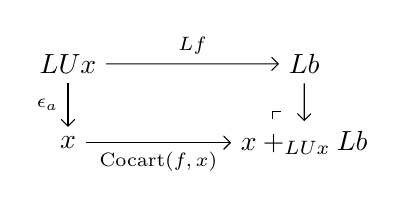
\begin{tikzpicture}
      \node (x) at (0,0) {$ x $};
      \node (po) at (3,0) {$ x+_{LUx}Lb $};
      \node (LUx) at (0,1) {$ LUx $};
      \node (Lb) at (3,1) {$ Lb $};
      \draw [cd] 
      (LUx) edge[] node[left]{$\epsilon_a$} (x)
      (LUx) edge[] node[above]{$Lf$} (Lb)
      (Lb) edge[] (po)
      (x) edge[] node[below]{$\Cocart(f,x)$} (po);
      \draw (2.6,0.3) -- (2.6,0.4) -- (2.7,0.4);
    \end{tikzpicture}
  \end{equation*}

% the below beautiful diagram was sacrificed for the sake of
% uniformity accross all diagrams and I don't know xypic
%
%
% \begin{displaymath}
%  \begin{tikzcd}
%    \L\U x \ar[r,"\L f"]\ar[d,"\varepsilon_a"']\ar[dr, phantom, "\ulcorner", pos=1] & \L b\ar[d,dashed] \\
%    x\ar[r,dashed] & x+_{\L\U x} \L b
%  \end{tikzcd}
% \end{displaymath}
where $\varepsilon\colon \L\U\Rightarrow1_\X$ is the counit of the adjunction $\L\dashv \U$. To verify this is a cocartesian lifting, first of all it must be mapped to $f$ via $\U$: if we apply $\U$ to the above square, using the facts that $\U\varepsilon_x=1_{a}$, $\U\L f=f$ (by Proposition \ref{prop:coreflection}) and $$\U (x+_{\L\U x}\L b)=\U x+_{\U\L\U x}\U\L b = a+_{a} b $$ since $\U$ strictly preserves pushouts, the resulting colimit diagram
  \begin{equation*}
    \begin{tikzpicture}
      \node (a1) at (0,0) {$ a $};
      \node (po) at (3,0) {$ a+_{a}Lb = b $};
      \node (a2) at (0,1) {$ a $};
      \node (b) at (3,1) {$ b $};
      \draw [cd] 
      (a2) edge[] node[left]{$1_a$} (a1)
      (a2) edge[] node[above]{$Lf$} (b)
      (b) edge[] node[right]{$1_b$} (po)
      (a) edge[] node[below]{$f$} (po);
      \draw (2.6,0.3) -- (2.6,0.4) -- (2.7,0.4);
    \end{tikzpicture}
  \end{equation*}

  % the below beautiful diagram was sacrificed for the sake of
% uniformity accross all diagrams and I don't know xypic
%
% 
% \begin{displaymath}
%  \begin{tikzcd}
%   a\ar[r,"f"]\ar[d,"1_a"'] & b\ar[d,dashed] \\
% a\ar[r,dashed] & a+_{a}b=b
%  \end{tikzcd}
% \end{displaymath}
is \emph{the} pushout of $f$ along the identity, namely $f$ due to our choice. Moreover, the universal property (cf.~Diagram \ref{fig:opfibration}) of the proposed cocartesian lifting follows from universality of pushouts thus the one direction of the proof is complete.
\end{proof}
%Christina: tried to see whether the converse is true, didn't go far. Remember that from previous prop we got it preserves initial for sure!

Combining \cref{prop:opfibtolari,prop:laritoopfib}, we establish certain conditions under which a Grothendieck opfibration corresponds to a rali and vice versa. %Christina: no more finite colimits: Steve said that for the strict case, this is more subtle than the ordinary case. Pretty sure that we don't wanna go into details there?
%Understand whether other such conditions could exist? More philosophically.

\begin{thm}\label{thm:mainthm}
Suppose that $\X$ and $\A$ have chosen pushouts and initial objects, and a functor $\U\colon\X\to\A$ strictly preserves them. Then $\U$ is a right adjoint left inverse if and only if $\U$ is an opfibration.
\end{thm}

% ===============================================================
% Street fibs and corefls. Examine relationship between.

\section{Street opfibrations and coreflectors}\label{Streetfibs}

In this section, we trod the same path as in Section \ref{sec:groth-fibs-ralis} but shed any strictness around preserving colimits by working with Street opfibrations instead of Grothendeick opfibrations and with reflectors instead of ralis

Generalising \cref{prop:opfibtolari}, we obtain the following. 

\begin{prop} \label{thm:street-opfib-to-corefl}
  Let $ \U \from \X \to \A $ be a Street opfibration. Then $ \U $ is a coreflector if its fibers have initial objects which are preserved by the reindexing functors.
\end{prop}

\begin{proof}
  We define $ \L $ exactly as in Proposition
  \ref{prop:opfibtolari}. 

  The unit of the adjunction $ \L \dashv \U $ is the
  identity $ a\to \U\L a = \U\bot_a = a $.  The
  counit is the initial map $ \bot_{\U x} = \L\U x \to
  x $.  The triangle identities are satisfied as
  well. The first is the composite
  \[
    \L a
    \xto{\L\eta_a}        \L\U\L a
    \xto{\epsilon_{\L a}} \L a
  \]
  which is given by $ \bot_a \to \bot_a \to \bot_a
  $.  The second is the composite
  \[
    \U x
    \xto{\eta_{\U x}} \U\L\U x
    \xto{\U\eta_x}    \U x
  \]
  which is given by $ \U x \to \U x \to \U x $.

  Because the unit of the adjunction is an
  isomorphism, $ \L $ is full and faithful
  \cite[{Prop.~1.3}]{gabrielzisman} making $ \U $ a
  coreflector.
\end{proof}

Applying Lemma \ref{lem:street-fibrewise-limits}, we can
transport the assumptions on the fibers to the base category
of our Street fibration.

\begin{cor}
  A Street opfibration is a reflector if the base
  category has and the functor preserves the (initial)
  terminal object.
\end{cor}

Generalising \cref{prop:laritoopfib}, we obtain the following result.

\begin{prop}
  \label{thm:corefl-to-street-opfib}
  Suppose that $ \U \from \X \to \A $ is a
  coreflector. Then $ \U $ is a Street opfibration
  if $ \X $ has pushouts and $ \U $ preserves them.
\end{prop}

\begin{proof}
  Fix an arrow $ f \from a \to b $ in $ \A $
  and an object $ x $ in the fibre of $ a $. We
  claim that $ \hat{f} $, defined as the pushout
  of $ \L f $
  along the counit $ \epsilon_x $
  \[
    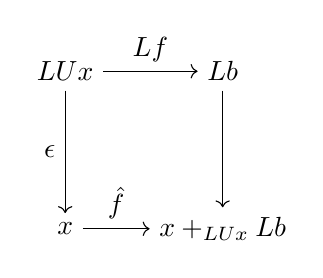
\begin{tikzpicture}
      \node (ul) at (0,2) {$ \L \U x $};
      \node (ll) at (0,0) {$ x $};
      \node (ur) at (2,2) {$ \L b $};
      \node (lr) at (2,0) {$ x +_{\L\U x} \L b$};
      \draw [->] (ul) to node [left] {$ \epsilon $} (ll);
      \draw [->] (ul) to node [above] {$ \L f $} (ur);
      \draw [->] (ll) to node [above] {$ \hat{f} $} (lr);
      \draw [->] (ur) to (lr);
    \end{tikzpicture}
  \]
  is the cocartesian lift. There is a string of
  isomorphisms
  \[
    \U ( x +_{\L\U x} \L b ) \cong
    \U x +_{\U\L\U x} \L b \cong
    \U x +_{\U x} b \cong
    b
  \]
  whose composite we call $ h $.  Then
  \[
    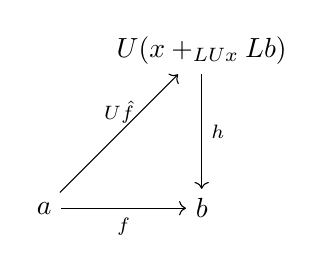
\begin{tikzpicture}
      \node (a) at (0,0) {$ a $};
      \node (b) at (2,0) {$ b $};
      \node (c) at (2,2) {$ \U ( x+_{\L\U x} \L b ) $};
      \path[->,font=\scriptsize]
      (a) edge node[below]{$ f $} (b)
      (a) edge node[above]{$ \U\hat{f} $} (c)
      (c) edge node[right]{$ h $} (b);
    \end{tikzpicture}
  \]
  commutes, and so $ \hat{f} $ is an appropriate
  lift. It remains to show that $ \hat{f} $ is
  cocartesian.

  Consider a $ \X $-arrow $ g \from x \to y $
  with a $ \A $-arrow
  $ \theta \from \U( x +_{\L\U x} \L b ) \to \U y $ so
  that $ \theta \U \hat{f} = \U g $.  Can we
  uniquely lift $ \theta $? Set up the diagram
  \[
    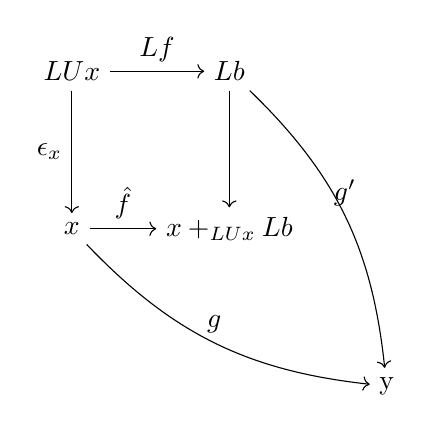
\begin{tikzpicture}
      \node (ul) at (0,2) {$ \L\U x $};
      \node (ll) at (0,0) {$ x $};
      \node (ur) at (2,2) {$ \L b $};
      \node (lr) at (2,0) {$ x +_{\L\U x} \L b$};
      \node (comp) at (4,-2) {y};
      \draw [->] (ul) to node [left] {$ \epsilon_x $} (ll);
      \draw [->] (ul) to node [above] {$ \L f $} (ur);
      \draw [->] (ll) to node [above] {$ \hat{f} $} (lr);
      \draw [->] (ur) to (lr);
      \draw [->] (ll) to [bend right=20] node [above] {$ g $} (comp);
      \draw [->] (ur) to [bend left=20] node [above] {$ g' $} (comp);
    \end{tikzpicture}
  \] 
  where $ g' \bydef \epsilon_y \L\theta \L h^{-1} $.
  To show the outer square commutes, it suffices
  to show that $ g' \L f $ and $ g \epsilon_x $
  have the same image under the adjunction homset
  correspondence.  We have
  \[
    g' \circ \L f =
    \epsilon_y \circ \L\theta \circ \L h \circ \L f
    \mapsto
    \U\epsilon_y \circ \U\L\theta \circ \U\L h
      \circ \U\L f \circ\eta_{ux}
    = \theta \circ h \circ f   
    = \theta \circ \U \circ \hat{f} 
    = \U g
  \]
  and 
  \[
    g \epsilon_x
    \mapsto
    \U g \circ \eta_{\U x}
    = \U g
  \]
\end{proof}

We now intersect the hypothesis of \cref{thm:street-opfib-to-corefl} and \cref{thm:corefl-to-street-opfib} to provide the main result of this section.

\begin{thm}
  \label{thm:main-theorem-street-version}
  Let $ U \from \X \to \A $ be a functor such that $ \A $ and $ \X $ have chosen initial objects and pushouts and $ U $ preserves them. Then $ \U $ is a coreflector if and only if $ \U $ is a Street opfibration.
\end{thm}

% ===============================================================
% Cats of fibs and adjs. Examine structure of relationship (todo later)



% ===============================================================
% Appendix. Choice of colimits.

\appendix{}

\section{Choice of colimits}
\label{sec:choice_of_colimits}

In what follows, and in particular for our main \cref{thm:mainthm}, we often require that certain colimits must be \emph{strictly} preserved. Although the strict preservation of colimits does not adhere to the principle of equivalence, it is required when working with Grothendieck fibrations. Moreover, in \cref{Streetfibs} we examine the non-strict context which then naturally matches to the notion of a Street fibration as discussed above.

In more detail, assuming the axiom of choice we can regard any category with colimits as having \emph{chosen} ones, in the sense of choosing a specific adjoint (from all isomorphic ones) to the constant diagram functor:
\begin{displaymath}
 \begin{tikzcd}[sep=.7in]
 \cat{C}\ar[r,pos=.6,"\Delta_\cat{C}"description]\ar[r,phantom,bend left=18,pos=.6,"\bot"]\ar[r,phantom,bend right=18,pos=.6,"\bot"] &  {[}\cat{J},\cat{C}{]}\ar[l,bend right,pos=.4,"\colim_\cat{J}"']\ar[l,bend left,pos=.4,"\lim_\cat{J}"]
 \end{tikzcd}
\end{displaymath}
Some categories, like $\Set$, even have a canonical choice corresponding to well-known constructions of colimits of sets. In general, a functor $F\colon\cat{C}\to\cat{D}$ between categories with colimits, for example, preserves them when the following diagram
\begin{equation}\label{eq:preservelimits}
  \begin{tikzcd}
\phantom{A}[\cat{J},\cat{C}]\ar[r,"\colim"]\ar[d,"{[\cat{J},F]}"']\ar[dr,phantom,"\cong"] & \cat{C}\ar[d,"F"] \\
\phantom{A}[\cat{J},\cat{D}]\ar[r,"\colim"'] & \cat{D}
  \end{tikzcd}
 \end{equation}
 commutes up to natural isomorphism.  The following two lemmas (due to
 Steve Lack) present two natural settings where functors between
 categories with chosen colimits strictly preserve them;
 evidently, such a thing is to be expected only when the colimits in the
 categories have been both previously constructed from chosen limits
 in some fixed category.
\begin{lem}\label{lem:Lack1}
 Suppose $\cat{C}$ is a category with chosen colimits of any class. Then for any two categories $\cat{A}$ and $\cat{B}$ and any functor $F\colon\cat{A}\to\cat{B}$ between them, the pre-composition functor
 \begin{displaymath}
  \begin{tikzcd}[row sep=.05in]
  F^*\colon[\cat{B},\cat{C}]\ar[r] & \;[\cat{A},\cat{C}] \\
  \;\;\;\;\left(\cat{B}\xrightarrow{H}\cat{C}\right)\ar[r,mapsto] & \left(\cat{A}\xrightarrow{F}\cat{B}\xrightarrow{H}\cat{C}\right)
  \end{tikzcd}
 \end{displaymath}
strictly preserves the chosen colimits.
\end{lem}
\begin{proof}
 This follows from the pointwise construction of colimits in functor categories.
\end{proof}

As a particular case, the following result concerns our motivating example.
\begin{cor}
There is a canonical choice of colimits in $\Grph$ inherited from those in $\Set$ so that the domain and codomain functors $\Grph\to\Set$ strictly preserve all colimits.
\end{cor}

\begin{proof}
  The domain and codomain functors, respectively $1^\ast$ and
  $2^\ast$, are built from the functors
  $1,2\colon\one{=}\{\bullet\}\longrightarrow\{1\rightrightarrows2\}{=}\two$.  Choosing the canonical colimits in $\Set$, by \cref{lem:Lack1} we obtain two functors
\begin{displaymath}
\begin{tikzcd}
 \Grph=[\two,\Set]\ar[r,shift left,"1^\ast"]\ar[r,shift right,"2^\ast"'] & \;[\one,\Set]=\Set
 \end{tikzcd}
\end{displaymath}
that strictly preserve them.
\end{proof}

The following case again follows from a construction of chosen limits in common ground; colimits adhere to a dual result.
\begin{lem}
Suppose $\cat{C}$ and $\cat{D}$ have chosen colimits and $F\colon\cat{C}\to\cat{D}$ is an arbitrary functor. Then the comma category $F\downarrow\cat{D}$ can be equipped with colimits in such a way that both projections $\cat{C}\leftarrow F\downarrow\cat{D}\to\cat{D}$ strictly preserve them.
\end{lem}

\begin{proof}
 This follows from the canonical construction of colimits in comma categories (see~\cite[\S 2.16]{Handbook1}).
\end{proof}

Finally, opfibrations form another class of functors that is notable when it comes to strictly preserving colimits. In more detail, we do not lose generality by assuming that a colimit preserving opfibration preserves strictly. Such a statement does not apply to arbitrary functors. This is due to the following lemma, which is a special case of a more general fact: the embedding of $\OpFib$ in the 2-category $\OpFib_{\sim}$ where 2-cells are squares filled with isomorphisms, is locally fully faithful and essentially surjective (also for fibs...references...\cite{Fib2Fib}?). We thank Claudio Hermida for these observations.
\begin{lem}\label{lem:isofactid}
 Suppose $\U$ and $\Q$ are opfibrations, and there is a natural isomorphism
 \begin{displaymath}
  \begin{tikzcd}
\X\ar[r,"H"]\ar[d,"\U"']\ar[dr,phantom,"\stackrel{\phi}{\cong}"] & \Y\ar[d,"\Q"] \\
\A\ar[r,"F"'] & \B
  \end{tikzcd}
 \end{displaymath}
Then $\phi$ factors as a commutative square composed by an isomorphism $\hat{\phi}$, as in
 \begin{displaymath}
  \begin{tikzcd}[row sep=.15in]
\X\ar[rr,bend left,"H"]\ar[rr,bend right,"\widehat{H}"']\ar[rr,phantom,"{\stackrel{\hat{\phi}}{\cong}}"description]\ar[dd,"\U"'] && \Y\ar[dd,"\Q"] \\
\hole \\
\A\ar[rr,"F"'] && \B
  \end{tikzcd}
 \end{displaymath}
\end{lem}
As a result, if $\U$ is an opfibration that preserves $\cat{J}$-colimits for some small $\cat{J}$, we can factor the natural isomorphism \cref{eq:preservelimits}, where the left leg is also a fibration, as
\begin{displaymath}
  \begin{tikzcd}[row sep=.15in]
{[\cat{J},\cat{X}]}\ar[rr,bend left,pos=.4,"\colim"]\ar[rr,bend right,pos=.4,"\widehat{\colim}"']\ar[rr,phantom,"\cong"description]\ar[dd,"{[\cat{J},\U]}"'] && \X\ar[dd,"\U"] \\
\hole \\
{[\cat{J},\cat{A}]}\ar[rr,"\colim"'] && \A
  \end{tikzcd}
 \end{displaymath}
essentially changing the choice of colimits in the total category and establishing that $Q$ now strictly preserves them. In a dual way, we may assume that any fibration strictly preserves chosen limits, if it preserves limits in the ordinary sense.



\bibliographystyle{plain}
\bibliography{references.bib}


\end{document}